\glsresetall

% \section{Abstract}
The number of publicly available microbiome samples is continually growing. As dataset size increases, bottlenecks arise in standard analytical pipelines. Faith’s phylogenetic diversity is a highly utilized phylogenetic alpha diversity metric that has thus far failed to effectively scale to trees with millions of vertices. Stacked Faith's Phylogenetic Diversity (SFPhD) enables calculation of this widely adopted diversity metric at a much larger scale by implementing a computationally efficient algorithm.  The algorithm reduces the amount of computational resources required, resulting in more accessible software with a reduced carbon footprint, as compared to previous approaches. The new algorithm produces identical results to the previous method. We further demonstrate that the phylogenetic aspect of Faith's PD provides increased power in detecting diversity differences between younger and older populations in the FINRISK study's metagenomic data.

\section{Introduction}

In microbiome research, particular attention is given to evaluating the diversity of microbes within samples \cite{McDonald2018-uf,The_Human_Microbiome_Project_Consortium2012-og,Thompson2017-pu}.  Alpha diversity (within sample diversity), in particular, can summarize the breadth of microbial diversity present in a sample. There are many examples of associations between various host factors and alpha diversity, including country \cite{McDonald2018-uf}, disease status \cite{Gevers2014-bs,Vazquez-Baeza2016-sq}, diet \cite{McDonald2018-uf}, and age \cite{Yatsunenko2012-wv} among many others \cite{Youngblut2019-pk,Jeffery2016-rc}.
Modern DNA sequencing instruments have enabled microbiome studies at the scale of tens of thousands of samples, which presents a computational challenge for metrics that rely on a phylogeny, such as Faith’s Phylogenetic Diversity (Faith’s PD) \cite{Faith1992-gh}. Faith’s PD is computed by summing the branch lengths (edge weights) of the phylogeny that exclusively represent the sequences contained in a biological sample. The amount of memory and number of necessary operations needed to calculate Faith's PD depends on the number of edges in the phylogenetic tree, as well as the number of samples in the underlying data table.
In today’s increasingly large and sparse datasets and meta-analyses, these phylogenetic trees and tables can exceed 100,000s of samples and millions of tree tips \cite{McDonald2018-qq}. Recent advances have enabled efficient computation of the UniFrac metric for beta diversity, which is also a metric computed over phylogenetic trees \cite{Lozupone2005-aj}. Specifically, Striped UniFrac \cite{McDonald2018-qq} improves upon previous UniFrac implementations \cite{Hamady2010-dg} by using space- and time-efficient tree data structures \cite{Cordova2016-vf} and reducing the number of vectors required to store intermediate scores in the tree. 
Additionally, the usefulness of techniques like Faith’s PD and UniFrac remains underexplored for metagenomics sequencing. Recent molecular protocol optimizations, such as SHOGUN \cite{Hillmann2018-vk}, have enabled the metagenomic characterization of large human cohorts  \cite{Salosensaari2020-tx,Borodulin2015-uz,Kaplan2019-yo}. In this context, the applicability of Faith’s PD has largely been limited by the technical difficulties associated with constructing phylogenies from metagenomic features \cite{Zhu2019-od}. Efforts like the Web of LIfe (WoL) \cite{Zhu2019-od} and Genome Taxonomy Database (GTDB) \cite{Parks2020-cg,Parks2018-gb} are now addressing this issue by providing a phylogenomic tree as part of their database releases that can be used for phylogeny-informed analysis.

Motivated by these advances in algorithms and resources for analyzing phylogenies, phylogenomic trees, and sparse data, we developed a new algorithm and implementation, Stacked Faith's Phylogenetic Diversity (SFPhD), for rapidly computing Faith’s PD. SFPhD produces identical results to those of previous algorithms for computing this metric while producing a speedup of up to 64x and requiring as little as 0.21\% of the memory in our benchmarks (Table~\ref{faiths_pd_table1}). The key advances of SFPhD are using a sparse matrix representation, an efficient tree structure, and partial aggregation of metric constituents. Our BSD-licensed implementation of this algorithm is available in the `unifrac' package (via PyPI and bioconda \cite{Gruning2018-fw}), which has 50,714 total conda downloads and 34,141 conda downloads since the introduction of SFPhD, as of the time of writing (May 13, 2021). The package produces a C/C++ shared library with Python bindings and is additionally linkable by any programming language (https://github.com/biocore/unifrac). Additionally, by investigating the previously documented relationship between age and bacterial richness of the gut microbiome \cite{De_la_Cuesta-Zuluaga2019-zr}, we demonstrate that accounting for phylogeny in metagenomic data can increase the statistical power for detecting group differences. 

% \usepackage{colortbl}

\begin{sidewaystable}
\caption[Average memory improvement and speedup of SFPhD compared to the reference implementation.]{Average memory improvement and speedup of SFPhD compared to the reference implementation.}
\label{faiths_pd_table1}
\centering
\begin{tabular}{|c|rrr|rrr|}
\hline
\multicolumn{1}{|l|}{} & \multicolumn{3}{l|}{Time (s)}                                                                                         & \multicolumn{3}{l|}{Memory (kbytes)}                                                                                      \\ \hline
\textbf{\# of Samples} & \multicolumn{1}{c|}{\textbf{skbio}} & \multicolumn{1}{c|}{\textbf{SFPhD}} & \multicolumn{1}{c|}{\textbf{Speedup (x)}} & \multicolumn{1}{c|}{\textbf{skbio}} & \multicolumn{1}{c|}{\textbf{SFPhD}} & \multicolumn{1}{c|}{\textbf{Improvement (x)}} \\ \hline
\textbf{1250}          & \multicolumn{1}{r|}{18.6}           & \multicolumn{1}{r|}{4.67}           & 3.98                                      & \multicolumn{1}{r|}{10001242.8}     & \multicolumn{1}{r|}{312815.6}       & 31.97                                         \\ \hline
\textbf{2500}          & \multicolumn{1}{r|}{32.8}           & \multicolumn{1}{r|}{5.12}           & 6.41                                      & \multicolumn{1}{r|}{19114300.4}     & \multicolumn{1}{r|}{313834.8}       & 60.91                                         \\ \hline
\textbf{5000}          & \multicolumn{1}{r|}{79.75}          & \multicolumn{1}{r|}{6.31}           & 12.64                                     & \multicolumn{1}{r|}{36727706.4}     & \multicolumn{1}{r|}{315124}         & 116.55                                        \\ \hline
\textbf{10000}         & \multicolumn{1}{r|}{270.34}         & \multicolumn{1}{r|}{8.76}           & 30.86                                     & \multicolumn{1}{r|}{75866321.6}     & \multicolumn{1}{r|}{317413.2}       & 239.01                                        \\ \hline
\textbf{20000}         & \multicolumn{1}{r|}{910.62}         & \multicolumn{1}{r|}{14.17}          & 64.26                                     & \multicolumn{1}{r|}{152783905.2}    & \multicolumn{1}{r|}{320837.6}       & 476.2                                         \\ \hline
\textbf{40000}         & \multicolumn{1}{l|}{*}              & \multicolumn{1}{r|}{25.58}          & \multicolumn{1}{l|}{N/A}                  & \multicolumn{1}{l|}{*}              & \multicolumn{1}{r|}{326895.2}       & \multicolumn{1}{l|}{N/A}                      \\ \hline
\textbf{80000}         & \multicolumn{1}{l|}{*}              & \multicolumn{1}{r|}{47.26}          & \multicolumn{1}{l|}{N/A}                  & \multicolumn{1}{l|}{*}              & \multicolumn{1}{r|}{339670}         & \multicolumn{1}{l|}{N/A}                      \\ \hline
\multicolumn{7}{l}{* No jobs were able to be completed with the prescribed resources.}
\end{tabular}
\end{sidewaystable}


\section{Results}
\subsection{Stacked Faith's PD provides a faster and memory-efficient implementation over the previous state-of-the-art algorithm.}

\begin{figure}[htbp]
\centering
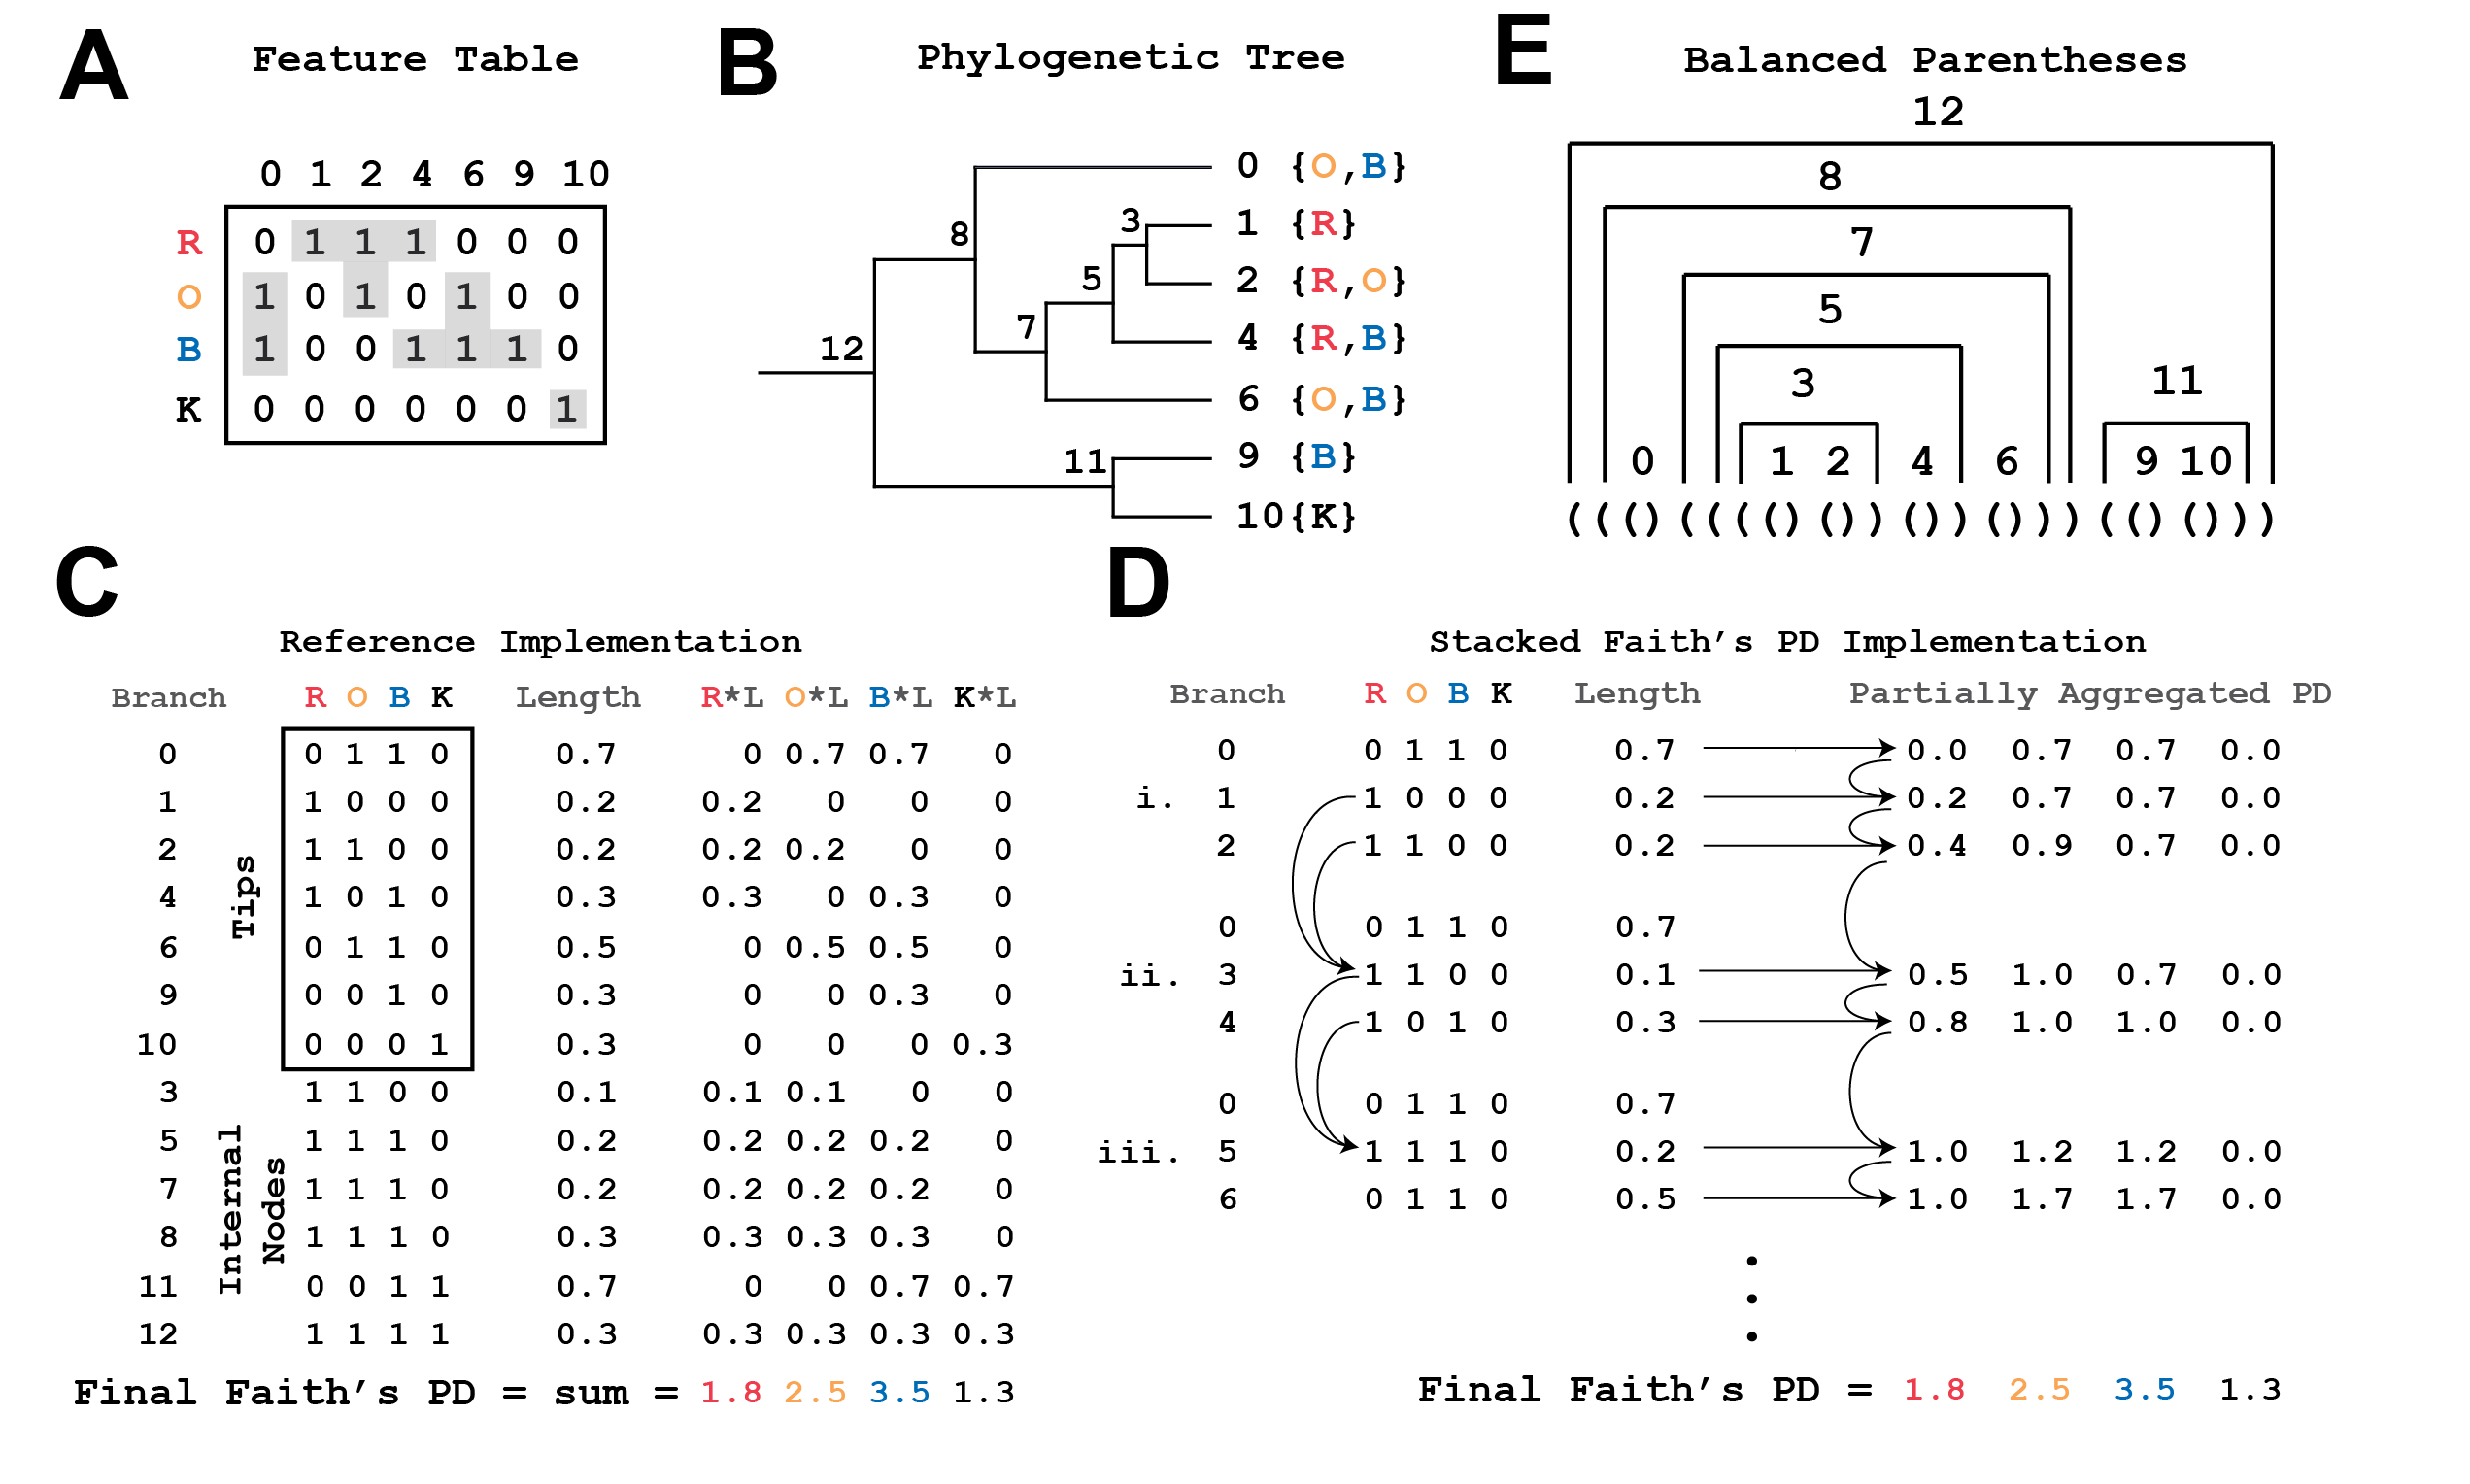
\includegraphics[width=\textwidth]{faiths-pd-figures/figure01.png}
\caption[Partially aggregating branch lengths reduces the space complexity of the algorithm.]{\textbf{Partially aggregating branch lengths reduces the space complexity of the algorithm.} (A) Faith's PD calculation depends on the representation of features present in samples. In the table, the letters (R, O, B, K) represent samples and the numbers (0, 1, 2, 4, 6, 9, 10) represent features. A 1 in an entry indicates the presence of a feature in the sample. SFPhD uses sparse table data structures, which reduce memory by only keeping track of the non-zero values in a matrix (highlighted in gray). (B) A mock reference phylogenetic tree is shown, with the features from (A) as tips. Labels for the samples from (A) are located next to tips that they contain. The nodes are labeled by their order in a post-order traversal of the tree. (C) Graphic depiction of the reference implementation's calculation of Faith's PD by first aggregating the presence/absence information for each branch in the tree, followed by multiplication by the branch lengths to get the metric constituents, and finally a sum over the entire branch ×metric constituent table. (D) Graphic representation of the execution of SFPhD. On the left, the stack of presence/absence information is shown at three points during the algorithm's execution (i, ii, ii). Each of these times shows the stack immediately before memory is freed. On the right, the state of the partially aggregated phylogenetic diversity (PD) is shown after each node is added to the stack. Each row represents the vector after a step in the algorithm. In practice, there is only one such vector. (E) The balanced parentheses representation for the phylogenetic tree from (B).}
\label{faiths_pd_fig1}
\end{figure}

We introduce Stacked Faith’s PD (SFPhD), a novel algorithm and implementation to compute Faith’s Phylogenetic Diversity that uses the structure of microbiome data along with other practical considerations to achieve decreased time and memory requirements. An example feature table is shown in Figure~\ref{faiths_pd_fig1}A, with a corresponding phylogenetic tree in Figure~\ref{faiths_pd_fig1}B. Note that for a given tree $\mathcal{T}$, Faith's PD can be expressed as
\begin{align}
PD_i = \sum_{j\in \mathcal{T}} I_{ij} \times \text{branchLen}_{j}(\mathcal{T})
\end{align}
where $PD_i$ is Faith's PD for sample $i$, $I_{ij}$ indicates if sample $i$ has any features that descend from node $j$, and $\text{branchLen}_j(\mathcal{T})$ indicates the length of the branch to node $j$ in the tree $\mathcal{T}$.

The previous state-of-the-art reference implementation (\href{http://scikit-bio.org/}{scikit-bio}) computes Faith's PD for a batch of samples by first fully computing $I_{ij}$. $I_{ij}$ is computed by traversing the entire phylogenetic tree in a post-order traversal and setting all $I_{ij}$ for a given node $j$ by determining the features present in all children of node $j$. Subsequently, the $I_{ij} \times \text{branchLen}_j(\mathcal{T})$ for all branches is calculated. The final results are obtained by summing over the branches for each sample (Figure~\ref{faiths_pd_fig1}C). However, this approach tends to use much more space than is actually needed.

Microbiome data are known to be sparse \cite{Martino2019-op,Kumar2018-or,Morton2017-bs}, i.e., of the entries in a data table, many are likely to be zero. This issue is exacerbated in large datasets, where many microbes are only observed in a handful of samples. In extreme cases, such as the table from \cite{McDonald2018-qq} with 113,721 samples rarefied at 500 sequences per sample, 0.0126\% of the entries are non-zero. Sparse representations have been used previously for storing microbiome data \cite{McDonald2012-go}, and have been applied for accelerating microbiome analyses \cite{McDonald2018-qq}, however, they have not been previously applied to Faith’s PD. We identified that a major downfall of the state-of-the-art implementation in scikit-bio is that it uses a full, dense table to represent all of $I_{ij}$ in memory at once. A key advancement of our approach is to use a sparse matrix implementation for storing information on the taxa present for each sample and feature (Figure~\ref{faiths_pd_fig1}A). 

Another key advancement is the partial aggregation of Faith's PD (Figure~\ref{faiths_pd_fig1}D). Note that the $I_{ij} \times \text{branchLen}_j(\mathcal{T})$, which we will call a metric constituent, can be added in any order, and that $I_{ij}$ only depends on the children of node $j$. Thus, if node $k$ is a child of node $j$, $I_{ik}$ is no longer needed once metric constituents for node $k$ have been computed and $I_{ij}$ is known. As a result, we can reduce the memory used to store $I_{ij}$ by traversing the phylogeny with a post-order traversal and freeing $I_{ik}$ after they are no longer needed. Furthermore, we can reduce the storage needed for the metric constituents keeping a running summation of them while traversing the tree. Thus, this approach reduces the expected space complexity for storing the metrics from $O(n k)$, to $O(n \log(k))$, where $n$ is the number of samples and $k$ is the number of vertices in the tree.

In addition to the algorithmic improvements, we have included a number of practical enhancements that improve the performance of the code. The phylogenetic tree (Figure~\ref{faiths_pd_fig1}B) is now represented as balanced-parentheses (Figure~\ref{faiths_pd_fig1}E); this structure has a lower memory footprint and a sequential memory representation which reduces the number of cache misses during a tree traversal \cite{Cordova2016-vf}. Finally, the software is written using C/C++ (with Python extensions using Cython, https://cython.org/) and builds upon the foundation established by Striped UniFrac \cite{McDonald2018-qq}. Reuse of this library facilitated our access to a much faster Newick format parser, which reduces the overhead when reading a tree from disk. These factors make for an improved expected and in-practice performance, despite the time complexity and worst-case memory complexity remaining the same.

To demonstrate the scalability of SFPhD, we used a collection of 307,237 public and anonymized private 16S rRNA V4 microbiome samples amounting to 1,264,796 phylogenetic tree tips (after rarefaction at 500 sequences per sample). The samples were retrieved using the redbiom command line interface \cite{McDonald2019-th} which queried a cache of public and anonymized private studies available in Qiita \cite{Gonzalez2018-ez}. Amplicon sequence variants (ASVs) were placed into the Greengenes \cite{Gonzalez2018-ez,McDonald2012-zv} phylogeny using SEPP \cite{Mirarab2012-jh}. Computing the full alpha diversity vector took SFPhD 1 hour and 5 minutes wall-clock time and required a maximum resident set size of less than 3 GB (see Methods for hardware details). In addition, we iteratively measured runtime and memory consumption for increasingly large random subsets of samples while fixing the size of the tree at 100,000 tips (Figure~\ref{faiths_pd_fig2} A,B). For the iteration with 20,000 samples, the memory usage of the reference implementation exceeded 150 GB and the process ran for over 15 minutes. Contrastingly, with SFPhD, the process took 14 seconds to execute and required less than 0.5 GB of memory. Additionally, using  Green Algorithms \cite{Lannelongue2021-vg}, we estimated the carbon footprint of the scikit-bio reference implementation on the 20,000 sample table be 12.84 g CO2e, whereas we estimated the carbon footprint of SFPhD would be 0.04 g CO2e in the United States, which is a 321-fold reduction in impact on global warming.

\begin{figure}[htbp]
\centering
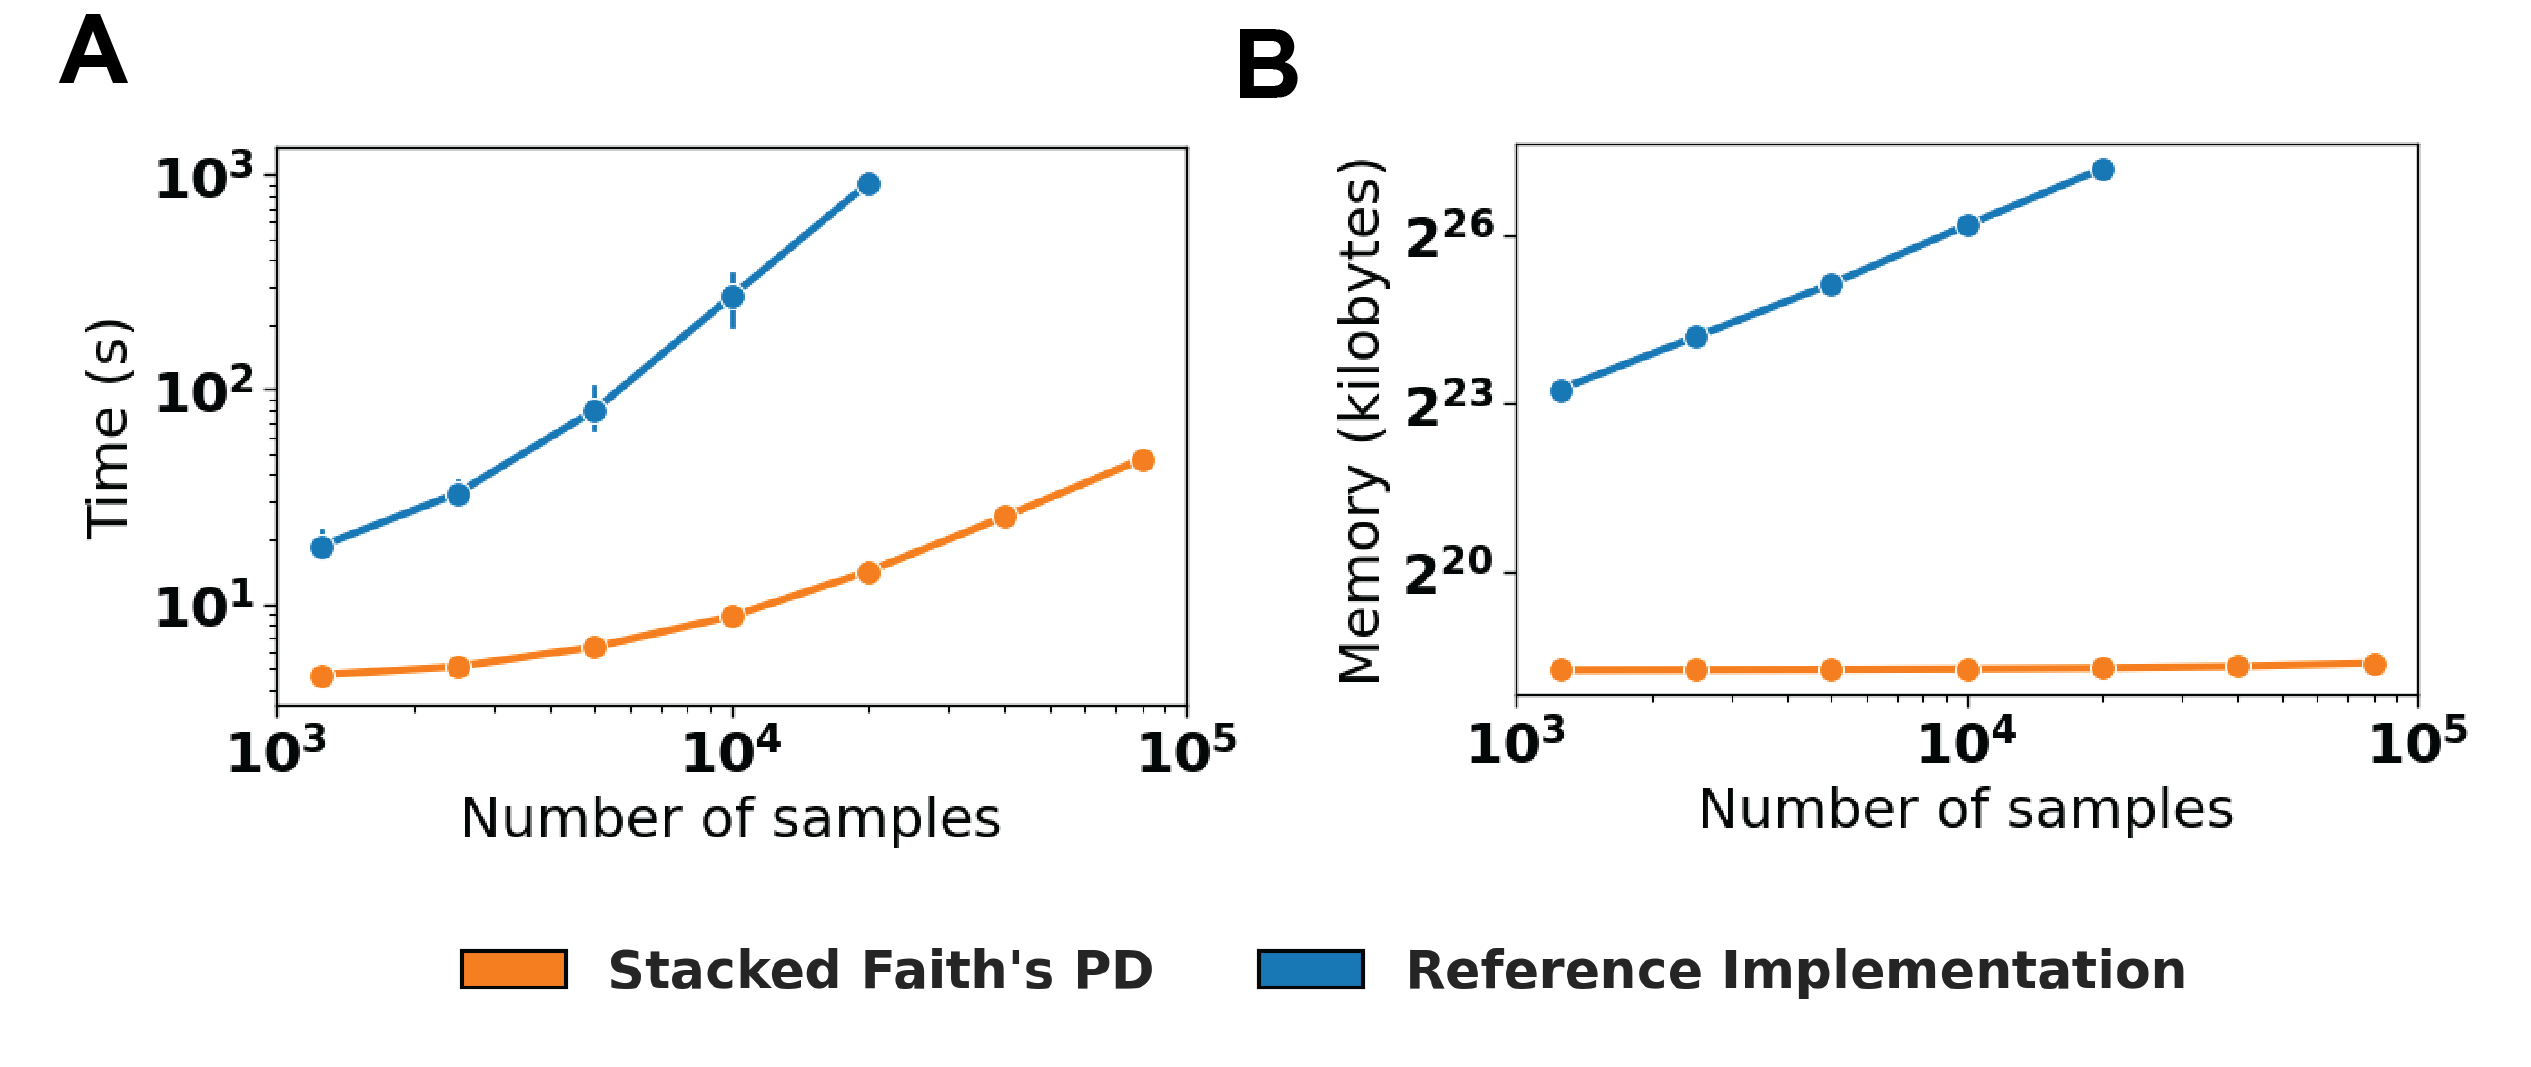
\includegraphics[width=\textwidth]{faiths-pd-figures/figure02.png}
\caption[SFPhD outperforms the reference implementation in terms of runtime and memory usage.]{\textbf{SFPhD outperforms the reference implementation in terms of runtime and memory usage.} (A) Runtime in seconds for computing Faith’s PD on datasets with thousands of samples and 100,000 tips in the phylogeny. Data is independently sub-sampled from a collection of 113,721 public samples in Qiita \cite{Zhu2019-od, Gonzalez2018-ez} as previously processed \cite{McDonald2018-qq}. Mean of n=10 repetitions with 95\% CI error bars. (B) Memory usage for the same experiment as in (A). For both a and b jobs were terminated if they exceeded 250 GB of memory.}
\label{faiths_pd_fig2}
\end{figure}

\subsection{Phylogenetic diversity is a suitable metric to analyze stool metagenomic samples}

To demonstrate SFPhD’s versatility and applicability to newer datasets, we reanalyzed 2,661 paired 16S rRNA and metagenomic data of stool samples from the FINRISK \cite{Borodulin2015-uz,Salosensaari2020-tx,Borodulin2017-sx} study (n=1,563 aged 60 and older, n=1,098 aged 35 and under) \cite{Salosensaari2020-tx,Borodulin2015-uz}. In this experiment, we select random subsets of the full sample set and compare each metric’s (Observed Features and Faith’s PD) ability to detect differences in mean alpha diversity distributions. For each step we randomly select $N$ paired 16S and metagenomic samples, and then compute the difference in mean alpha diversity between samples taken from younger adults (under 35 years) and older adults (over 60 years) together with an empirical p-value. For both 16S and metagenomics, the alpha diversity of younger adults is lower than in older adults. In metagenomics, but not in 16S sequencing, Faith’s PD provides improved statistical power over a phylogenetically-agnostic alternative (Figure~\ref{faiths_pd_fig3} A,B). With 16S data, the difference between the two metrics is subtle (Figure~\ref{faiths_pd_fig3}A). In both cases, the statistical power increases as the number of samples grows. With metagenomic data, the number of observed features shows a weaker effect compared to Faith’s PD regardless of the number of samples (Figure~\ref{faiths_pd_fig3}B). Unlike 16S datasets (5,600 features), metagenomic datasets (1,700 features) are resolution-limited by the reference databases. Whereas the nature of amplicon sequence variants (ASVs) allow for a broader feature space that can capture age-differences without the need for a phylogeny. 

\begin{figure}[htbp]
\centering
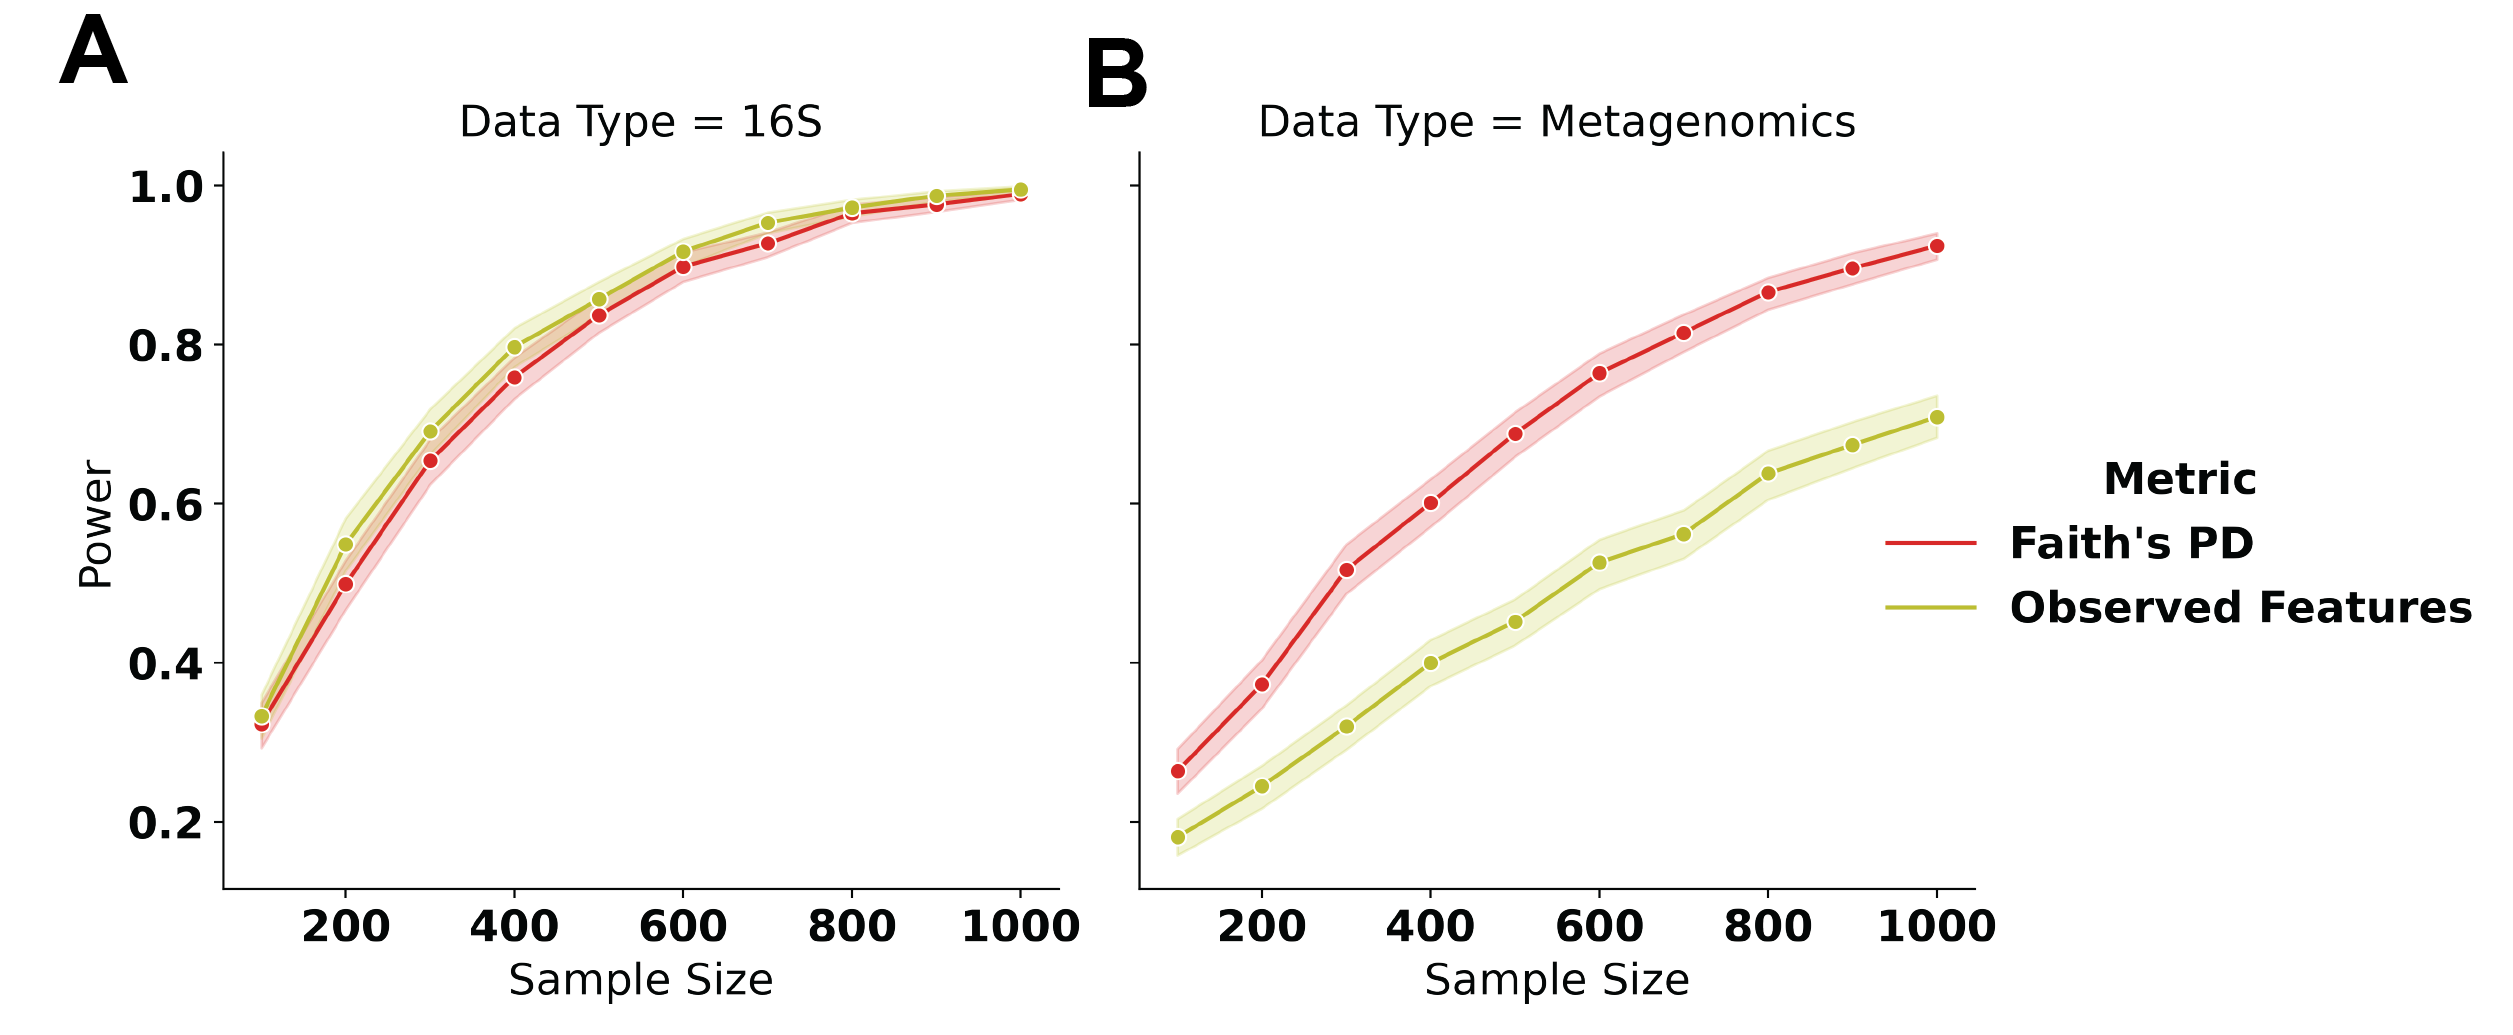
\includegraphics[width=\textwidth]{faiths-pd-figures/figure03.png}
\caption[Phylogenetic diversity provides increased statistical power to differentiate age groups in shotgun metagenomics but not in 16S rRNA sequencing.]{\textbf{Phylogenetic diversity provides increased statistical power to differentiate age groups in shotgun metagenomics but not in 16S rRNA sequencing.}  (A) Statistical power to differentiate young adults from old adults in two alpha diversity metrics at different sample sizes using 16S rRNA sequencing in the FINRISK cohort. (B) Same as (A) but for shallow shotgun metagenomic sequencing.}
\label{faiths_pd_fig3}
\end{figure}

By computing the log of the likelihood ratio of older to younger adult samples present for each branch in the WoL phylogenomic tree \cite{Zhu2019-od}, we were able to identify portions of the WoL tree responsible for the increase in phylogenetic diversity (Figure~\ref{faiths_pd_fig4}B). From this analysis, we found that the majority of the tree is comparably represented in young and old adult samples. However, we also found two clades where older adult samples were more prevalent than younger adult samples (Clade 1 has a log ratio bounded with an 80\% confidence interval of [1.20, 1.45] and Clade 2 has an 80\% confidence interval of [0.55, 0.74]). Clade 1 corresponds to a majority of \textit{Lactobacillales} genomes, and Clade 2 corresponds to \textit{Proteobacteria} genomes. The branches in Clade 1 primarily have a large log likelihood ratio, indicating that the features across the entire clade are more likely to be found in samples from older adults. However, the internal branches in Clade 2 additionally have low log likelihood ratios, indicating that the enrichment of features in older adults is not completely consistent across the entire clade. Lastly, although not confined to a few clades, there are several tips (e.g. \textit{Staphylococcus aureus}, \textit{Bavariicoccus seileri}, \textit{Nitratireductor indicus}, and \textit{Campylobacter ureolyticus}) in the phylogeny that are only associated with younger adults.

\begin{figure}[htbp]
\centering
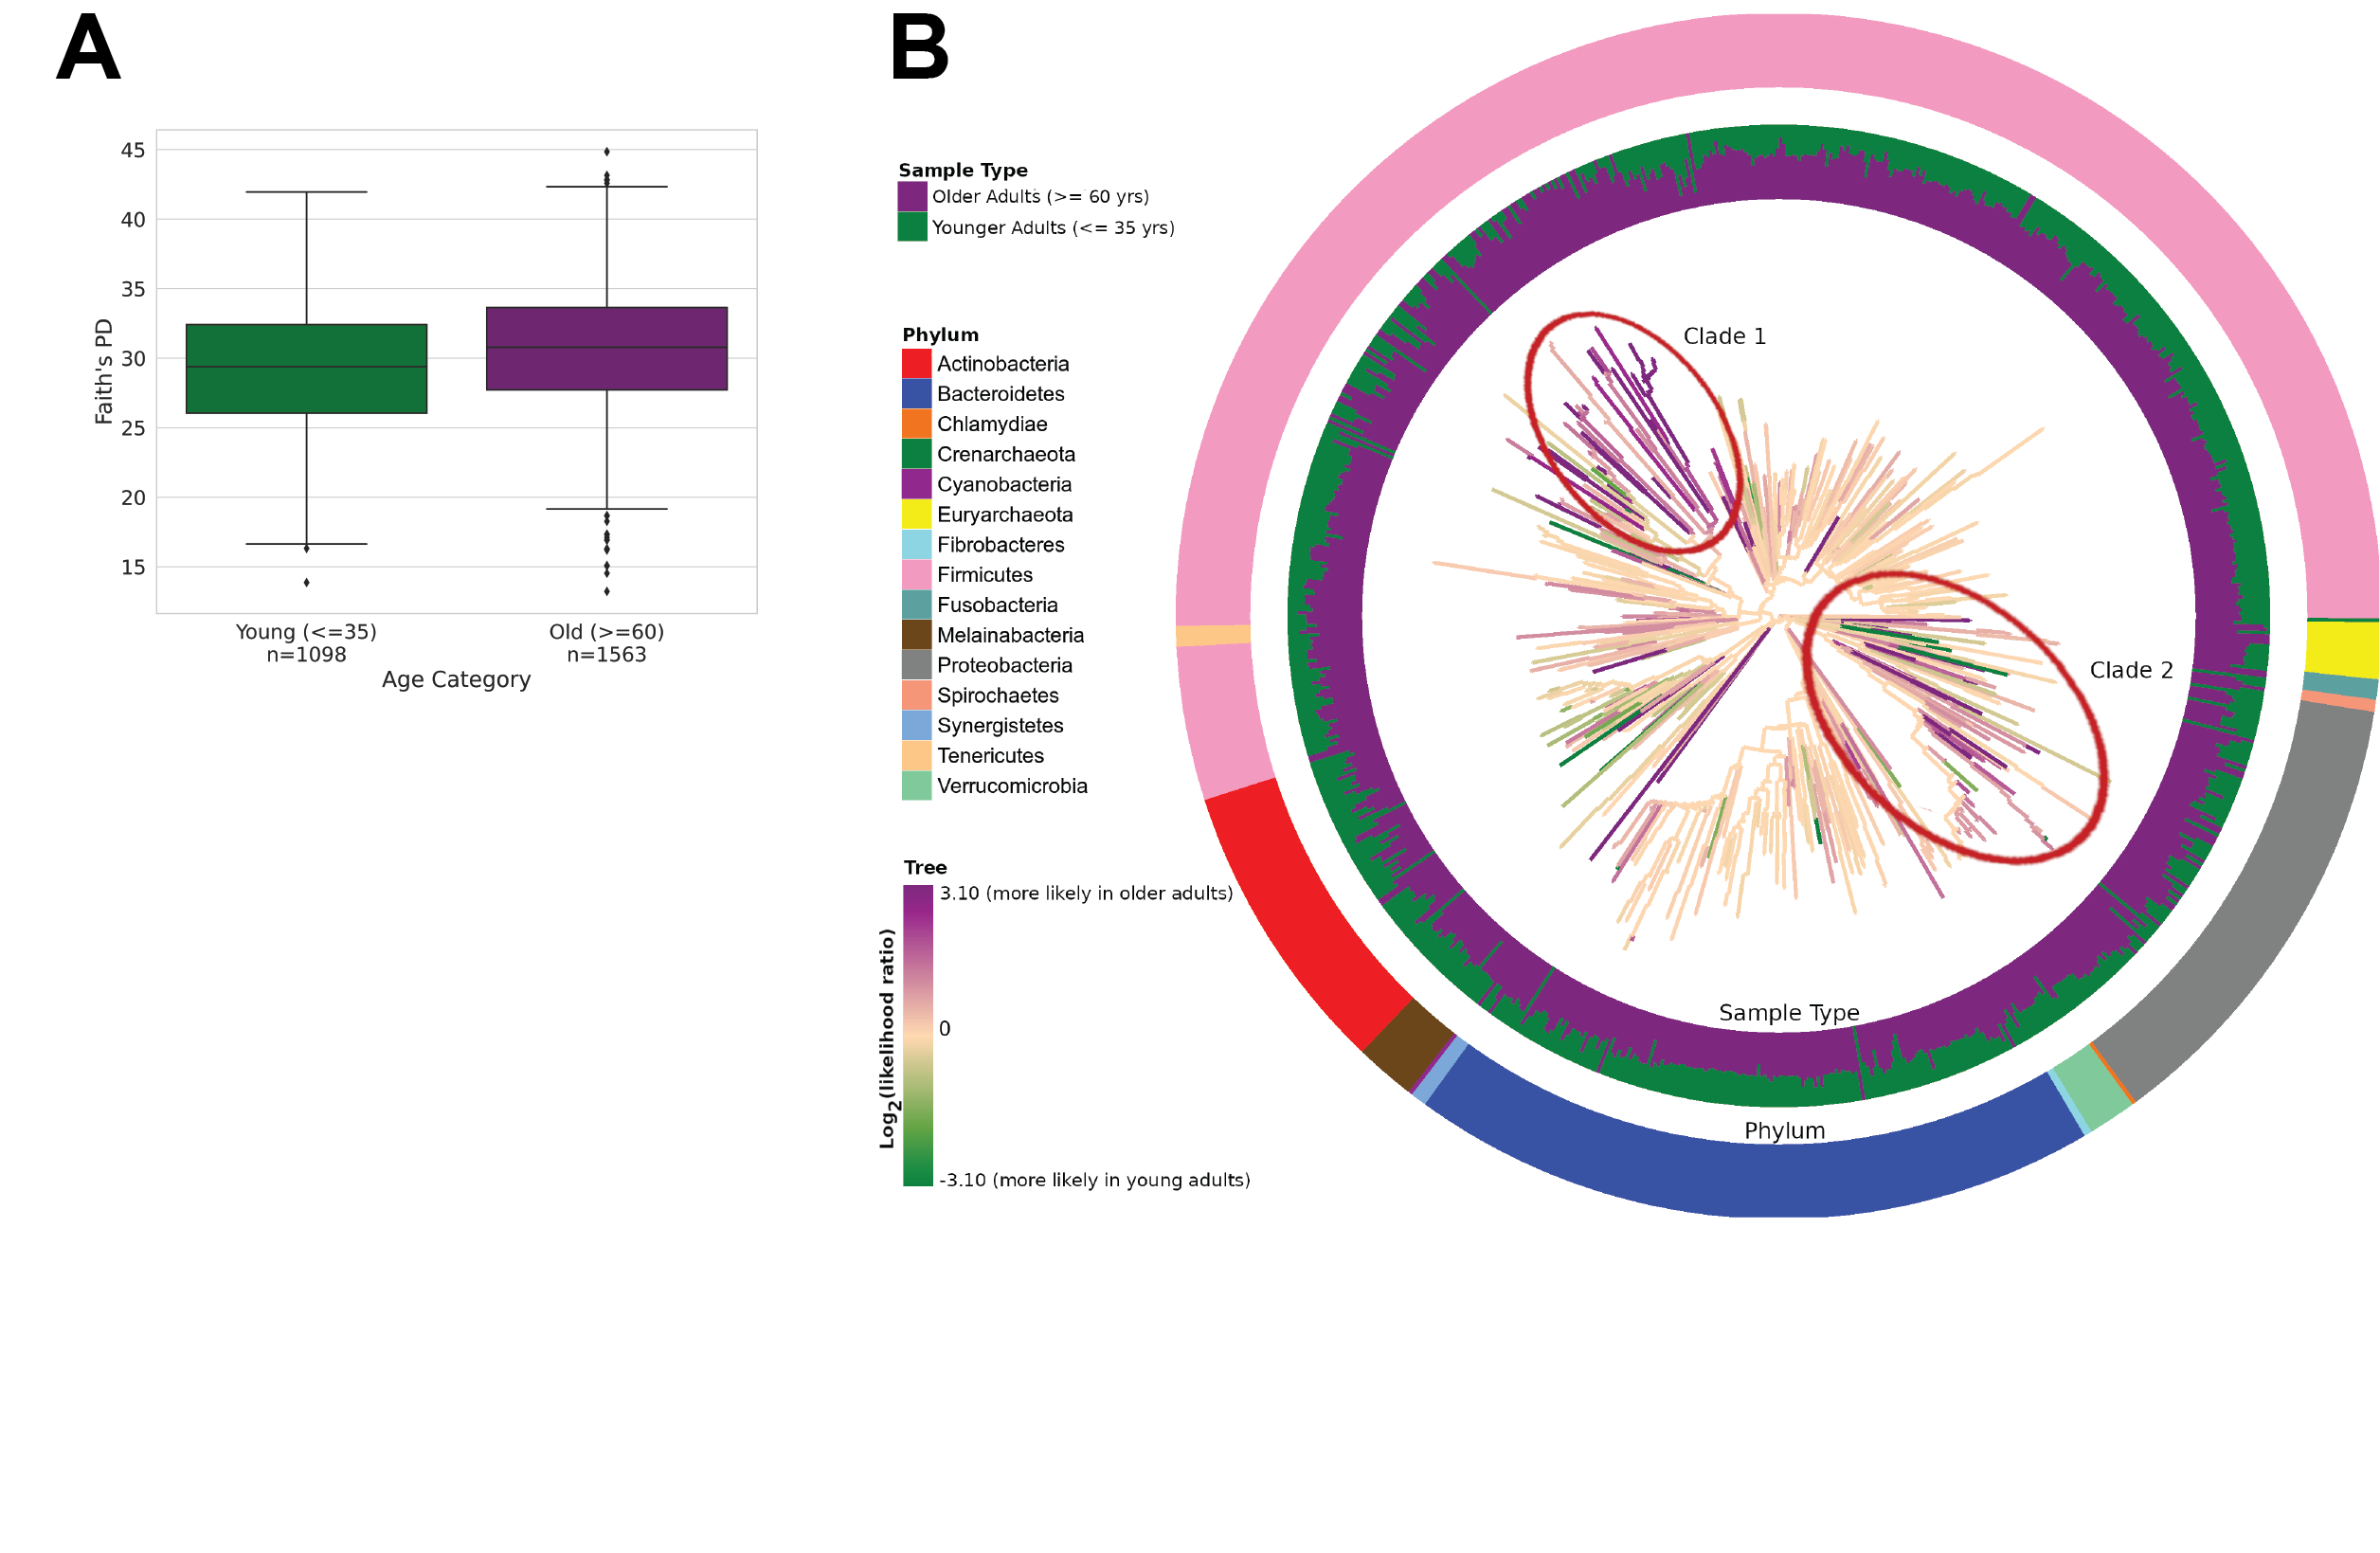
\includegraphics[width=\textwidth]{faiths-pd-figures/figure04.png}
\caption[Phylogenetic tree colored by age-group log of the likelihood ratio of older to younger adults per node]{\textbf{Phylogenetic tree colored by age-group log of the likelihood ratio of older to younger adults per node.}  (A) Distribution of Faith's PD by age group on the full dataset. (B) Web of Life (WoL) Phylogenetic tree with branches colored by the log of likelihood ratio of old adults compared to young adults in descendants of the branch, for the FINRISK dataset. The inner circle is colored by the log of likelihood ratio of older adults compared to younger adults in the tips of the tree. The outer circle is colored by the phylum of the taxon represented by each tree tip. Red ellipses mark two clades enriched for samples from older individuals.}
\label{faiths_pd_fig4}
\end{figure}

\section{Discussion}
By accounting for the relationship between features in a dataset, Faith’s PD is able to mitigate issues with sparsity and heterogeneity common to modern `omics’ datasets. Although this metric was first introduced 30 years ago, the underlying algorithm for computing this metric had largely remained unchanged. In this paper we demonstrated that our novel algorithm, SFPhD, performed efficiently on datasets with hundreds of thousands of samples and millions of tree tips.

An important aspect of SFPhD’s underlying algorithm is substituting calculation of the full presence/absence table over the phylogeny, for a tree traversal that partially aggregates diversity values and frees presence/absence information when no longer needed. The result is a high-performance implementation that demonstrates improved scaling, with the number of samples in the input dataset. Much of the engineering work here was facilitated by the balanced parenthesis tree implementation provided in the UniFrac package \cite{McDonald2018-qq}. Therefore, we believe that increasing the availability of efficient and flexible data structures for bioinformatic analyses, is likely to accelerate and facilitate the development of novel analytical methods. In a broader sense, this is similar to the impact of NumPy’s \cite{McDonald2018-qq,Harris2020-vb} N-dimensional array in image processing, machine learning, neuroscience, and other fields. 

In addition, in a stool metagenomic study Faith’s PD demonstrates increased statistical power compared to Observed Features for differentiating younger from older subjects based on their microbial communities. In this context, we show that while the choice of alpha diversity metric did not make a significant difference for the 16S dataset in this study, Faith's PD consistently provided increased statistical power for determining age-based differences in the shotgun metagenomic sequencing data. While this metric was originally developed to analyze data with vastly different statistical and biological properties, its use here demonstrates the versatility and applicability behind measuring diversity using a tree. Although we show the utility of SFPhD in large and complex microbiome studies, the underlying implementation is not tied to a particular molecular technology. Thus, we envision that this implementation will be relevant to fields outside of microbiology, like nutrition and metabolomics research, that only recently began adopting trees for analytical tasks \cite{Tripathi2021-wf,Johnson2019-nx}.  

\section{Methods}
\subsection{Construction of benchmarking tables}
Data for the benchmarking in this study were subsampled from a BIOM table of 113,721 and 761,003 ASVS, which is composed of studies aggregated from several large sources of publicly available microbiome data in Qiita \cite{Amir2017-sk,Gonzalez2018-ez}. This data table was produced as in \cite{McDonald2018-qq}. The data was subset by uniformly randomly sampling the desired number of ASVs and samples from the table. Ten different tables were created for each number of samples and ASVs. The insertion tree from \cite{McDonald2018-qq} was collapsed to only contain sequences that were selected to be included in the given subsampled table.
The table with 307,237 public and anonymized private 16S rRNA V4 microbiome samples and 1,264,796 phylogenetic tree tips was also prepared as in \cite{McDonald2018-qq}, but included samples with private sequencing data from Qiita.

\subsection{Benchmarking time and memory estimates
}

The SFPhD implementation available in the python package unifrac v0.10.0 was used. The reference implementation uses the Faith's PD implementation from scikit-bio v0.5.4.

All methods were run single-threaded on shared compute nodes that were not running other compute tasks. The nodes all had Intel(R) Xeon(R) CPU E5-2640 v3 @ 2.60GHz processors. A job was terminated if it exceeded 6 hours of wall time or 250 GB of memory (system max). Space was tracked using GNU Time. Time for both implementations was tracked with a python wrapper script. The time needed to parse data is not included in the scikit-bio timings, but is included in the SFPhD timings, due to the lack of access to this information in the unifrac interface. This is acceptable given that it results in a conservative estimate of the speedup with SFPhD.

\subsection{Carbon footprint estimation}
The Green Algorithms interface \cite{Lannelongue2021-vg} was used to estimate the Carbon Dioxide equivalent ($\text{CO}_2\text{e}$) of the benchmarked methods. The Intel(R) Xeon(R) CPU E5-2640 v3 CPUs used in benchmarking have a Thermal Design Power (TDP) per core of the  11.25 TDP / core.

\subsection{FINRISK processing}
The 16S rRNA data were demultiplexed, quality filtered, and denoised with deblur \cite{Amir2017-sk}.The Greengenes \cite{McDonald2012-zv} 13.8 with a clustering level of 99\% was used as the reference phylogeny for open-reference feature picking with SEPP \cite{Mirarab2012-jh}. ASVs with a total frequency fewer than 10 were discarded, and the table was then rarefied to a sampling depth of 1000 reads/sample. The resulting table and insertion tree were used for calculation of Faith's PD.
The shotgun metagenomic data were trimmed and quality filtered using Atropos \cite{Didion2017-pl}. They were aligned to the WoL database using SHOGUN pipeline (v1.0.8) with a Bowtie2 alignment option. A table was generated from the alignments using the OGU workflow \cite{Zhu2021-ap}.  OGUs with a total frequency fewer than 10 were discarded, and the table was then rarefied to a sampling depth of 1000 reads/sample. The WoL phylogenomic tree \cite{Zhu2021-ap,Zhu2019-od} was used for Faith's PD.
Both tables were filtered to include only samples from individuals 35 and younger (younger criteria) or 60 and older (older criteria).

\subsection{Power estimation for mean difference in alpha diversity}
For a given $N$ (shown on horizontal axis in Figure~\ref{faiths_pd_fig3} A,B), the FINRISK processed samples matching the younger/older criteria were sampled to this depth. On the subsampled data, the difference in mean alpha diversity between younger and older adults $\bar{d}$, was computed. A null distribution, $\hat{D}$, was generated by repeating 1000 repetitions of shuffling the  age category associated with an alpha diversity and recomputing the difference of mean alpha diversity between the groups. The p-value was computed by finding the percentile of $\bar{d}$ in $\hat{D}$.
This test procedure was repeated for 1000 repetitions. The power for $N$ is estimated as the proportion of tests found significant at $\alpha = 0.05$.

\subsection{Phylogenetic Visualization}
Tree was visualized using EMPress \cite{Cantrell2021-mx}. A node in the tree was considered old if its $\text{age}_{\text{log}} > 0$ and young if its $\text{age}_{\text{log}} < 0$.

\section{Data Access}
The data used for benchmarking Faith's PD timing and memory usage are available as per the Striped UniFrac paper \cite{McDonald2018-qq}. The code for the benchmarking is available on GitHub (https://github.com/biocore/faiths-pd-benchmarking). The data and code needed for benchmarking the FINRISK metagenomics data are also available on GitHub. The SFPhD code is available in the unifrac python package (https://github.com/biocore/unifrac). 

\section{Acknowledgements}
This work was supported in part by IBM Research AI through the AI Horizons Network, the Center for Microbiome Innovation at UC San Diego, the Academy of Finland grant 321351 and the Emil Aaltonen Foundation (to T.N.), the National Institutes of Health grant R01ES027595 (to M.J.), the Academy of Finland grants 321356 and 335525 (A.S.H), the Academy of Finland grant 295741 (L.L.). MI was supported by the Munz Chair of Cardiovascular Prediction and Prevention. VS was supported by the Finnish Foundation for Cardiovascular Research. 

Chapter~\ref{chapter_faiths_pd}, in full, is a reprint of the material as it appears in ``Efficient computation of Faith's phylogenetic diversity with applications in characterizing microbiomes.'' George Armstrong, Kalen Cantrell, Shi Huang, Daniel McDonald, Niina Haiminen, Anna Paola Carrieri, Qiyun Zhu, Antonio Gonzalez, Imran McGrath, Kristen Beck, Daniel Hakim, Aki S Havulinna, Guillaume Méric, Teemu Niiranen, Leo Lahti, Veikko Salomaa, Mohit Jain, Michael Inouye, Austin D Swafford, Ho-Cheol Kim, Laxmi Parida, Yoshiki Vázquez-Baeza and Rob Knight. \textit{Genome Research 31}, 2021. The dissertation author was the primary investigator and the first author of this paper.
